%!TEX root = ../authorinstr.tex

\section{Introduction}
TODO:: current state of the art stuff, mention OpenAI, Alpha-Go,..
TODO:: Research question


Designing an optimal controller for an environment, given a goal can be a complex task. Reinforcement learning techniques exist to adress these tasks by learning a policy that results in choosing optimal actions in a given state. State and action spaces can be either descrete or continueos. Descrete 


In the field of Reinforcement Learning (RL) an agent learns to behave in an environment to maximize an received reward.


In initial stages the agents performs randomly to explore the consequences of chosen action at a given state.
New algorithms are being developed and recently new environments arise for agents to engage in. 

Reinforcement learning is a machine learning technique which allows for agents to autonomously learn relatively complex behaviour
in a variety of applications such as such as playing backgammon \cite{tesauro2002programming} or chess \cite{baxter1999knightcap},
real life quadripedal walking \cite{kohl2004policy}, or autonomous simulated driving \cite{}. \\

With reinforcement learning an agent is placed in an environment in a state where it can execute a number of actions. Each
action the agent takes in a state entails a reward or a punishment for the agent as well as bringing it to a new state.
By maximizing tt's reward the agent gradually learns the value of each state (either by keeping track of this value in a
lookup table, or when the environment is to complex for this to be feasible, by approximating the value function for the
environment with a function approximator such as a multi-layer perceptron - MLP), allowing it to autonomously learn the optimal policy
for its environment. \\
When they were first developed reinforcement learning algorithms were designed to deal with discretized state and action
spaces. In real life however state spaces aren't discritized and although action spaces can be, this is not ideal as different
actions may require different levels of discritization to be accurate to get the desired reward. Furthermore the required level
of discritization can not be known in all 11cases, and having to discover it is time intensive \cite{van2007reinforcement}. %citatie naar de cacla paper
This potential problem can be solved by keeping the state and action space continuous in the environment representation of the agent. \\
Several new reinforcement learning algorithms and adaptations of existing reinforcement algorithms were developed to model continuous
state and action spaces. In this paper we will benchamark one such algorithm, named Neural Fitted Actor Critic (NFAC), which was develeped in August 2016 \cite{zimmer2016neural}
against two established (at the time of the writing of this paper) continuous reinforcement learning algorithms, named CACLA (Continuous Actor Critic Learning Automaton)
\cite{van2007reinforcement}
and SARSA (State Action Reward State Action) adapted for continuous state- and action-spaces \cite{nichols2014application} with gradient descent (referred to in this paper as GD-SARSA). \\
First a formal background will be given on connectionist reinforcement learning with the use of MLP's as function approximators,
and on extending this to continuous state- and action-spaces. In the methods section the three algorithms that are compared
 in this paper the implementation of these algorithms are explained in detail. After that setup of the experiments will be discussed.
Finally the results will be presented and evaluated, and the final conclusions will be drawn regarding NFAC compared to CACLA and GD-SARSA.

\begin{figure}[t]
 \centering 
    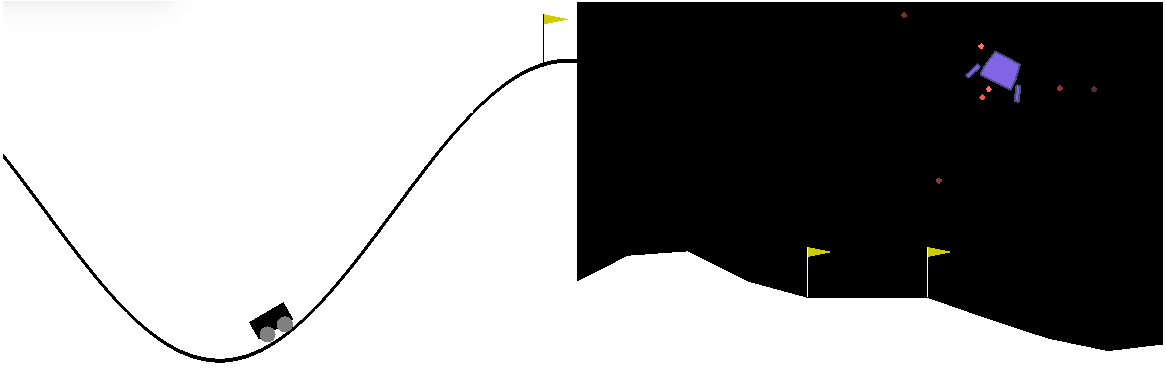
\includegraphics[width = 0.7\columnwidth]{figs/mountainlunar.png}
 \caption{Left: MountainCar Environment, Right: LunarLander Environment.}
\label{fig:mountainlunar}
\end{figure}
